\chapter{Monte Carlo Simulation of Physics Processes at ATLAS}
\label{chap:MCSimulation}

\indent Simulated event samples are used to model the signal and background processes in this analysis. A full list of the samples that are used is given in Appendix~\ref{App:DatasetList}.

\begin{table}[htpb]
  \centering
  \small
  \begin{tabular}{ccccccc}
    Process & Generator & fragm./hadron. & PDF set  & UE Tune & Cross section order\\
    \hline 
    \hline
    SUSY Signal & {\sc MadGraph5\_aMC\/@NLO} & {\sc Pythia} 8 & NNPDF2.3 & A14 & LO  & \\ 
    $t\bar{t}$ & {\sc Powheg-Box} v2 & {\sc Pythia} 6 & CT10  & {\sc Perugia 2012} & NLO & \\ 
    Single top & {\sc Powheg-Box} v2 & {\sc Pythia} 6 & CT10  & {\sc Perugia 2012} & NLO & \\ 
    $W/Z$+jets & {\sc Sherpa} 2.2.1 & {\sc Sherpa}  & NNPDF3.0NNLO & Default & NLO & \\ 
    Diboson & {\sc Sherpa} 2.2 & {\sc Sherpa} & CT10 & Default & LO\\ 
    $t\bar{t}+V$ & {\sc MadGraph5\_aMC\/@NLO} & {\sc Pythia} 8 & NNPDF3.0NNLO & A14 & NLO \\ 
    \hline
    \hline
  \end{tabular}
  \caption{Overview of the nominal simulated samples. }
  \label{tab:mc_samples1}
\end{table}

\section{Signal Monte Carlo Generation}
\label{sec:MC:Sig}

\indent For the stop signal, the matrix element (ME) of the hard scattering interaction are calculated using {\sc MadGraph5\_aMC\/@NLO}.  Up to two additional QCD partons are included in the ME calculation, making the total hard scattering process $pp /rightarrow {\stop}\bar{\stop} + j + j $.  The ME calculation is performed to leading order accuracy (LO).  \\

\indent The stop decays are treated differently depending on the mass splitting between the stop and its decay products.  The resulting decays are be seen in the Feynman diagrams shown in figure \ref{fig:feynDiagModels}. \\

\begin{figure}[htb]
  \begin{center}
    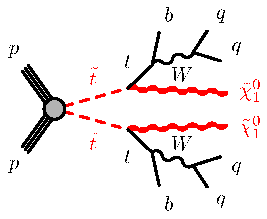
\includegraphics[width=0.25\textwidth]{figures/feynDiag/stst-bqqbqqN1N1-tt.eps}\hspace{0.05\textwidth}
    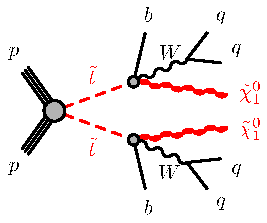
\includegraphics[width=0.25\textwidth]{figures/feynDiag/stst-bqqbqqN1N1-3body.eps}\hspace{0.05\textwidth}
\end{center}
\caption{The decay topologies of the signal models considered depending on the mass splitting between $\stop$ and $\ninoone$, a real top maybe produced in the 2 body decay $\stop\rightarrow t\ninoone$, or virtually through a three body decay ${\stop}\rightarrow bW\ninoone$}
\label{fig:feynDiagModels} 
\end{figure}

\indent If $m_{\stop} - m_{\ninoone} \ge m_{\top}$, then the top can be produced on shell. \pythiaeight\ perform 2 body ${\stop} \rightarrow \top \ninoone$ decay and subsequent decays of the top.  $m_{\top}$ is set to $172.5 \gev$.  This process has the advantage in that is is much computationally faster when compared to decaying the stops as part of the ME calculation.  However it has the disadvantage of effectively assuming that the stop width is zero.  The zero stop width assumption was found to differ from the true stop width case by less then $5$ percent in the distributions of all relevant kinematic variables.  The nominal stop width in the simplified model is $1/10$ the width of the top and so the stop width represent only a small smearing on the distribution of $m_{\top}$ and $\MET$ compared of the one produced by the top width. \\

\indent If $m_{\stop} - m_{\ninoone} < m_{\top}$, then the top must be produced off shell.   \pythiaeight\ cannot perform the 3 body $\stop \rightarrow b W \ninoone$ or 4 body $\stop \rightarrow b f f \ninoone$ decays where the "f" stands for the fermions that result from a $W$ decay.  Instead we use \madspin\ to perform the $\stop \rightarrow b ff \ninoone$ decay.  \madspin\ can perform 3 body and 4 body decays with off shell virtural particles as long as the decay are ultimately a series of 2 body decays.  \madspin\ performs the decays in a timely manner compared to calculated the decay within the ME.   In this case, \madspin cannot calculate the spin correlations between the two stops but this is not a problem because the stops are scalar particles so no spin correlations exist between the two. \\

\indent In addition to the ME calculation and stop decays, the parton shower (PS) and hadronization of jets are simulated with \pythiaeight\ with the {\sc EvtGen} v1.2.0 program as afterburner.  The matching between the matrix element and parton shower jets is preformed with the CKKW-L prescription.   The matching scale is set to $1/4$ the mass of the stop.. \\

\indent The internal structure of the proton is modeled with the NNPDF3.0NNLO parton distribution function (PDF) set with A14 set as the underlying event tuned parameters (UE tune).\cite{NNPDF3.0}  The A14 tune optimizes over 10 parameters that vary the amount of ISR, FSR and multiple parton interactions.  The variations are reduced to a 5 variable subset that is found to cover experimental observables.\cite{Pythia8tunes}  Variable 1 mainly cover variation in the modeling of the underlying events.  Variable 2 mainly cover variation in jet structure and variable 3a, 3b and 3c cover different variations of ISR and FSR production.  All 5 variations are used to quantify the theoretical uncertainties associated with parton shower and multiple parton interactions and are added in quadrature.\\

\indent Signal cross sections are calculated to next-to-leading order in the strong coupling constant with the resummation of soft gluon emission added to next-to-leading-logarithmic accuracy (NLO+NLL).\cite{stopXsec}  An envelope of cross section predictions is produced using different PDF sets and factorization and renormalization scales.  The nominal cross section and the uncertainty are then taken from the median and 1 sigma fluctuations around the median within the envelope.  \\

\indent A 2D grid of signal samples is generated to cover the stop and neutralino mass phase space that we maybe sensitive to.  Stop masses between 200 and 700 GeV are generated separated in $m_stop$ by 50 GeV.  For each Stop mass, five different ${\Delta}m = m_{\stop} - m_{\ninoone}$ are simulated: ${\Delta}m = m_{\top} - 82.5 \gev, m_{\top} - 52.5 \gev, m_{\top} - 22.5 \gev, m_{\top} - 7.5 \gev, m_{\top}+0.5 \gev,  m_{\top}+15.5 \gev, m_{\top}+27.5 \gev$.  An extra row of $m_{\stop} = 225 \gev$ samples is also produced to quantify the bound of sensitivity at low stop masses. \\

\section{SM Background Monte Carlo Generation}
\label{sec:MC:Bkg}

\subsection{Standard Model $\ttbar$ Monte Carlo Generation}

\indent The nominal ttbar samples are generated using \textsc{Powheg-Box}v.2.  The matrix element calculation is computed to NLO accuracy and includes the $pp \rightarrow \ttbar + j$ process where the $j$ is an one additional emitted parton.  The top quark mass is set to $172.5 \gev$ and the proton substructure is modeled by the NLO CT10 PDF set \cite{CT10} for the hard scattering process.  The hard scattering renormalization and factorization scales are set to the generator default of $\sqrt{(m_{\top})^2 + (p_{T \top})^2}$.  \\

\indent \pythia 6 version 6.427 simulates the parton shower, hadronization and underlying event.  We use the Perugia 2012 tune \cite{Perugia2012} and the corresponding leading order CTEQ6L1 PDF set \cite{CTEQ6L1} in \pythia 6.  The resummation damping factor or $h_{damp}$ which is one of the parameters used by \textsc{Powheg} to control the ME and PS matching and the amount of high-$\pt$ ISR/FSR, is set to $m_{\top}$. \\

\indent ttbar cross-sections are calculated to NNLO accuracy in the strong coupling constant with the resummation of soft gluon emissions added to NNLL accuracy using the \textsc{Top++v2.0} program. \cite{topXsec}  Again an envelope of cross-sections is produced for different PDF sets including MSTW2008NNLO, CT10 NNLO and NNPDF2.3 NNLO.  Variations in the renormalization and factorization scales, strong coupling constant, and top quark mass are also included in the envelope.  The median of envelope is taken as the nominal ttbar cross-section and the 1 sigma variation in the envelope is taken as the ttbar cross-section uncertainty.  \\

\indent In addition to the total cross-section uncertainty, a number of ttbar samples are produced to study the variation in the shapes of ttbar kinematic distributions. \\
\indent  A radHi and radLo sample are produced to study the variation in the total amount of ISR/FST $\pt$.  These samples are also produced with \textsc{Powheg+\pythia6} but have different renormalization and factorization scales (x0.5 to radHi and x2 to radLo). The radHi sample also has the $h_{damp}$ parameter that help control the matching between PS and ME increased from the nominal $m_{top}$ to x2 $m_{top}$. \\

\indent We study the variation of the parton shower simulation using a \textsc{Powheg+Herwigg++} ttbar sample.  The hard scattering ME calculation has not changed from the nominal.  The PDF used for the ME calculation is still NLO CT10 and the calculation is still performed with \textsc{Powheg-Box}v.2 with the $h_{damp} = m_{\top}$.  However the PS, fragmentation and hadronization is now performed with \textsc{Herwigg++} with the CTEQ6L1 PDF set \cite{CTEQ6L1} with the UE-EE-5 parameter tune. \\

\indent Variation in the hard scattering ME calculation are studied by comparing the nominal to a sample generated with \sherpa~\cite{sherpa}.  The same CT10 PDF set is used for sherpa and the nominal sample. \\ 

\indent Non overlapping samples that are filtered according to $\MET$ are generated to increase statistics at high $\MET$ where our analysis resides.  These samples are then merged to form a  continuous distribution in \MET. \\

\subsection{Standard Model Single Top Monte Carlo Generation}

\indent Like the nominal ttbar sample, the nominal single top samples are also simulated with \textsc{Powheg-Box}v.2 and interfaced to \pythia 6 for hadronization and parton showering, with CT10 PDF set and using the Perugia 2012 set \cite{Perugia2012} of tuned parameters. \\

\indent Unlike the ttbar samples, single top samples are produced separately according to production channels.  Three production channels exist including the s-channel, t-channel and the Wt channel.  The largest contribution to our analysis comes from the Wt channel.  \\

\indent The NLO calculation of the $pp \rightarrow Wt$ includes contributions from $ pp \rightarrow \ttbar \rightarrow \top + b + W$.  However $ pp \rightarrow \ttbar \rightarrow \top + b + W$ is already included in our simulation of ttbar and including it here would be double counting.  We can subtract out the ttbar contribution at either the level of amplitude (DR scheme) or at the level of matrix elements (DS scheme).  Subtracting at the matrix element level also remove any potential interference between the single top $pp \rightarrow Wt$ and ttbar $ pp \rightarrow \ttbar \rightarrow \top + b + W$ processes.  Subtracting at the amplitude level does not remove those interferences.  Both schemes violates formal gauge invariance and there isn't a consensus on the correct procedure.  We generate two sets of Wt channel single top samples with the two schemes.  The nominal single top sample is generated with the DR scheme and another sample is generated with the DS scheme.  We to compare the difference between the two samples to quantify the uncertainty due to the single top and ttbar interference terms. \\

\indent RadHi and radLo samples are also produced for all channels to study the variation in single top ISR and FSR emissions.  These samples are also produced with \textsc{Powheg+\pythia6} but have different renormalization and factorization scales (x0.5 to radHi and x2 to radLo). The radHi sample also has the $h_{damp}$ parameter that help control the matching between PS and ME increased from the nominal $m_{top}$ to x2 $m_{top}$. \\

\indent We study the variation of the parton shower simulation using \textsc{Powheg+Herwigg++} single top samples.  The hard scattering ME calculation has not changed from the nominal.  The PDF used for the ME calculation is still NLO CT10 and the calculation is still performed with \textsc{Powheg-Box}v.2 with the $h_{damp} = m_{\top}$.  However the PS, fragmentation and hadronization is now performed with \textsc{Herwigg++} with the CTEQ6L1 PDF set \cite{CTEQ6L1} with the UE-EE-5 parameter tune. \\

\subsection{Standard Model $\Wjets$ and $\Zjets$ Monte Carlo Generation}

\indent $\Wjets$ and $\Zjets$ are generated with the \sherpa v2.2.1 program.  The matrix element are calculated for the vector boson (V) plus 0,1, and/or 2 additional partons at NLO accuracy and 3, and/or 4 additional partons at LO accuracy.  \\

\indent The ME calculation is merged with \sherpa\ parton show according to the MEPS@NLO prescription.  The proton substructure is modeled with the NNPDF3.0 NNLO PDF set and the PS tuning defined by \sherpa.  \\

\indent  Systematic variations include a 7 point variation of the renormalization and factorization scales.  The variations are used to quantify the theoretical uncertainty on our modeling of the $\Wjets$ and $\Zjets$. \\

\indent  The $\Wjets$ and $\Zjets$ samples are generated in multiple non-overlapping slices of vector boson pt and b-jets and c-jets presence.  The samples are then merged later to form a continuous distribution covering all phase space.  This allows us to generate higher MC statistics in the region of phase space that is relevant to our analysis, the high-$\pt$ region with the presence of b and/or c-jets. \\

\subsection{Standard Model \ttbar+V Monte Carlo Generation}

\indent \ttbar+V where V is a $W$ or $Z$ boson samples are generated using {\sc MadGraph5\_aMC\/@NLO} with the NNPDF3.0NLO PDF set. The matrix element calculation is performed to NLO accuracy. The parton shower, fragmentation, and hadronization is simulated using \pythiaeight\ with the underlying event tune A14.  Variations in the hard scattering ME calculation are studied by generating another sample using \sherpa and comparing its results to the nominal sample.  Variation in renormalization and factorization scales are also produced. \\

\subsection{Standard Model $\ttbar+\gamma$ Monte Carlo Generation}

\indent $\ttbar+\gamma$ samples are generated using {\sc MadGraph5\_aMC\/@NLO} with the NNPDF3.0NLO PDF set. The matrix element calculation is performed to NLO accuracy. The parton shower, fragmentation, and hadronization is simulated using \pythiaeight\ with the underlying event tune A14.  The sample only simulates events with a filter for high photon $\pt$.  This sample is then merged with the nominal ttbar sample to form the $\ttbar+\gamma$ sample.  The events with high $\pt$ photons in the nominal ttbar samples are removed by a filter to avoid double counting. \\

\subsection{Standard Model Diboson Monte Carlo Generation}

\indent dibosons samples are generated with \sherpa v2.2 using CT10 PDF set. 

\section{Detector Simulation}
\label{sec:MC:DET}

\indent Two types of detector simulations were used.  \geant 4 is used to perform the detector simulation for all background samples including ttbar, \Wjets, \Zjets, single top, $\ttbar+V$, $\ttbar+\gamma$, and dibosons.  For signal MC, a fast simulation framework is used in the interest of computing time.  In fast simulation the majority of the detector are still simulated with \geant 4 with the exception of jets in the electromagnetic and hadronic calorimeter.  Instead of simulating individual particle showers in the calorimeters, a predetermined parameterized description of the showers are used instead.  The fast simulation framework was validated against full \geant 4 simulation for several selected signal samples and found to agree in observed kinematics.  \\

\indent Groups within ATLAS that measure the detector and reconstruction performance may recommend reweighing of different MC depending on better or worse then expected performance of different reconstruction algorithms. Corrections are applied through reweighing to correct for known differences between data and simulation for the lepton trigger and reconstruction efficiencies, momentum scale, energy resolution, isolation, and for the efficiency of identifying jets originating from the fragmentation of $b$-quarks, together with the probability for mis-tagging light-flavor and charm quarks as recommended by ATLAS performance groups. \\

\section{Pile-Up Simulation}
\label{sec:MC:PileUp}

\indent Because the LHC is operating at such high instantaneous luminosities, there are a on average 23 proton-proton interactions per bunch crossing.  Most of these interactions have low amounts of momentum transfer between the protons and are called minimum-bias interactions.  These interactions are also called pile-up interactions.  In addition to the hard scattering interaction of interest, all MC samples are produced with a varying number of simulated minimum-bias interactions.  The distribution of the number of additional overlaid minimum bias interactions is reweighed so that the distribution of the number of reconstructed of vertexes matches between data and MC.  \\

